%% WiNN manuscript for Bioinformatics
%% WiNN corrections use the frozen permutation-calibration development release 0.1.7.9999.

\documentclass[namedate,webpdf,modern,large,nocrop]{oup-authoring-template}

\graphicspath{{figures/}{figures/main_panels/}}
\newcommand{\societylogo}{}

\usepackage{array}
\usepackage{booktabs}
\usepackage{microtype}
% Keep the OUP running-header rules out of a column-width paragraph.
% This fixes template output-box warnings without changing body dimensions.
\usepackage{etoolbox}
\makeatletter
\patchcmd{\@oddhead}{\rule{\textwidth}{1\p@}}{\hrule width\textwidth height1\p@}{}{}
\patchcmd{\@evenhead}{\rule{\textwidth}{1\p@}}{\hrule width\textwidth height1\p@}{}{}
\setlength{\headheight}{19pt}
\makeatother

\usepackage{multirow}

\ifdefined\WiNNReviewCopy
  \usepackage[mathlines,switch]{lineno}
  \usepackage{setspace}
\fi

\begin{document}

\journaltitle{Bioinformatics}
\copyrightyear{2026}
\pubyear{2026}
\appnotes{Original Paper}
\firstpage{1}

\title[WiNN for selective technical correction]{WiNN enables selective correction of run-order drift and batch effects in metabolomics data}

\author[1,2,6]{Tanmay Tanna}
\author[2]{Yirui Zhang}
\author[2]{Anja Sjöström}
\author[4]{Franco Giulianini}
\author[2,6]{Malte Londschien}
\author[2]{Antoine Jeanrenaud}
\author[2,5,8]{André Kahles}
\author[7]{Mitchell P. Levesque}
\author[2,5,6,8,$\ast$]{Gunnar Rätsch}
\author[2,3,4,$\ast$]{Olga Demler}

\address[1]{\orgdiv{Department of Biosystems Science and Engineering}, \orgname{ETH Zürich}, \orgaddress{\country{Switzerland}}}
\address[2]{\orgdiv{Department of Computer Science}, \orgname{ETH Zürich}, \orgaddress{\country{Switzerland}}}
\address[3]{\orgdiv{Harvard T.H. Chan School of Public Health}, \orgaddress{\state{MA}, \country{USA}}}
\address[4]{\orgdiv{Brigham and Women's Hospital, Harvard Medical School}, \orgaddress{\state{MA}, \country{USA}}}
\address[5]{\orgdiv{Medical Informatics}, \orgname{University Hospital Zürich}, \orgaddress{Zürich, \country{Switzerland}}}
\address[6]{\orgname{AI Center, ETH Zürich}, \orgaddress{Zürich, \country{Switzerland}}}
\address[7]{\orgdiv{Department of Dermatology}, \orgname{University Hospital Zürich and Medical Faculty, University of Zürich}, \orgaddress{\country{Switzerland}}}
\address[8]{\orgname{Swiss Institute for Bioinformatics}, \orgaddress{\state{Lausanne}, \country{Switzerland}}}

\corresp[$\ast$]{Corresponding authors. \href{mailto:raetsch@inf.ethz.ch}{raetsch@inf.ethz.ch}; \href{mailto:odemler@bwh.harvard.edu}{odemler@bwh.harvard.edu}; \href{mailto:olga.demler@inf.ethz.ch}{olga.demler@inf.ethz.ch}}

\abstract{
\textbf{Motivation:} Mass-spectrometry (MS) intensities are affected by feature-specific run-order drift and batch effects. Existing approaches often require densely interleaved quality-control (QC) samples or correct all features, risking removal of biological signal.\\
\textbf{Results:} We developed White Noise Normalization (WiNN), a selective correction framework that applies drift and batch correction only to features showing evidence of technical variation. WiNN tests each feature for run-order drift and residual batch effects, corrects detected drift using conservative spline fits, and does not require QC identities. In simulated data with technical effects, WiNN reduced root mean squared error from 0.293 to 0.074, outperforming five established methods on all ground-truth measures. In public and clinical datasets, it removed most batch-related structure while preserving replicate agreement and biological group structure, and increased cross-batch sample matching from 46.3\% to 71.4\% and from 75.2\% to 85.8\%. WiNN relies on appropriate experimental randomization and is limited when acquisition order or batch assignment is confounded with biological covariates.\\
\textbf{Availability and Implementation:} WiNN is an open-source \texttt{R} package (GPL-3). The permutation-calibrated development version is at \url{https://github.com/ratschlab/winn}; the preceding release is on CRAN at \url{https://CRAN.R-project.org/package=winn}.\\
\textbf{Contact:} \href{mailto:raetsch@inf.ethz.ch}{raetsch@inf.ethz.ch}; \href{mailto:odemler@bwh.harvard.edu}{odemler@bwh.harvard.edu}; \href{mailto:olga.demler@inf.ethz.ch}{olga.demler@inf.ethz.ch}\\
\textbf{Supplementary Information:} Supplementary data are available at \textit{Bioinformatics} online.
}

\keywords{metabolomics; mass spectrometry; batch correction; run-order drift; normalization; generalized additive models}

\maketitle

\ifdefined\WiNNReviewCopy
  \onecolumn
  \fontsize{12pt}{18pt}\selectfont
  \doublespacing
  \linenumbers
\fi

\section{Introduction}
\label{sec:introduction}

Metabolomics using mass spectrometry (MS) provides a systems-level readout of biochemical state and is widely used for clinical biomarker discovery, disease stratification and mechanistic studies. Samples are acquired sequentially, and signal intensities can drift with acquisition order owing to instrument equilibration, ion-source contamination, carryover and temperature changes. Sample preparation, handling and changes in instrument state can also introduce shifts between batches \citep{Dunn2011,Brunius2016ClusterDrift,Wehrens2016BatchCorr}. Such technical variation can be feature-specific and sometimes exceed the biological differences being studied.

Established methods to address this include empirical-Bayes adjustment for batch effects when batch labels are available, QC-based smoothing approaches or machine-learning models that use reference samples to learn and remove run-order drift \citep{Johnson2007ComBat,Luan2018StatTarget,Fan2019SERRF,Han2022TIGER}, and study-sample regression methods that estimate drift without QC samples \citep{Wehrens2016BatchCorr,Rusilowicz2016Background}. These methods generally correct every metabolite without testing for the corresponding technical effect. Improved QC precision or reduced batch structure can therefore come at the expense of biological variation \citep{Kim2021hRUV}.

Randomizing samples along acquisition order during experimental design is essential. Biological groups and covariates should be balanced across batches and mixed along acquisition order \citep{Dunn2011,Jonsson2015}. If a biological phenotype is confounded with acquisition order or batch, technical and biological variation cannot be disentangled without additional assumptions. When samples are appropriately randomized, the goal of correction is to remove detectable technical variation while retaining biological differences among study samples. Widely used technical performance measures, such as QC coefficient of variation (CV), residual drift and batch separation, quantify technical variation but cannot establish whether biological differences have been preserved.

We developed White Noise Normalization (WiNN) to make correction conditional on evidence of technical variation. Under a randomized acquisition design, WiNN tests each metabolite for run-order dependence, detrends selected profiles while preserving segment means, then tests for and adjusts residual batch effects. Conservative smoothers limit removal of sample-to-sample variation. WiNN builds on the white-noise testing and selective spline correction of WiNNbeta \citep{Demler2024WiNNbeta}, adding a separate test for residual batch shifts, robust preprocessing, dilution normalization and automatic segmentation. It can also operate without QC identities. We compared WiNN with five established methods using simulations, a clinical cohort with cross-plate replicates, and four public datasets with replicates, biological groups or covariates.

\section{Materials and methods}
\label{sec:methods}

\subsection{Design principle and WiNN workflow}

WiNN assumes that acquisition order and batch assignment are independent of the biological variables of interest. Under this design, dependence of metabolite intensity on acquisition order can indicate technical drift. Regularly alternating sample types can also produce such dependence without instrumental drift (Section~\ref{sec:stress}). WiNN operates on a non-negative metabolite intensity matrix, requires acquisition order and optionally uses batch labels and QC identities.

For each metabolite, WiNN first shrinks extreme values using a median absolute deviation (MAD)-based rule, followed by a $\log(1+x)$ transformation. Within each batch or inferred run segment, WiNN measures serial dependence with the Ljung--Box statistic \citep{LjungBox1978} and calibrates selection using 999 shared permutations of acquisition order. The largest statistic across metabolites in each permutation provides a familywise-adjusted permutation $P$-value. Selected profiles are detrended using smooth, penalized curves, with simpler fits used when necessary, while preserving the segment mean \citep{Cleveland1979LOESS,Wood2017GAM}. WiNN then tests each metabolite for remaining batch differences, applies Benjamini--Hochberg (BH) adjustment \citep{BenjaminiHochberg1995} and adjusts selected features while preserving the overall metabolite mean. Finally, optional probabilistic quotient normalization (PQN) adjusts unusually large sample-level dilution differences, leaving typical dilution factors unchanged \citep{Dieterle2006PQN}. Supplementary Methods S1 gives the equations, model hierarchy and safeguards. For prespecified segments and parameters, random permutation sampling controls drift-selection familywise error within each segment under joint exchangeability of the prepared null profiles; ordered biology or scheduled sample types can violate this assumption (Section~\ref{sec:stress}).

\begin{figure*}[t]
\centering
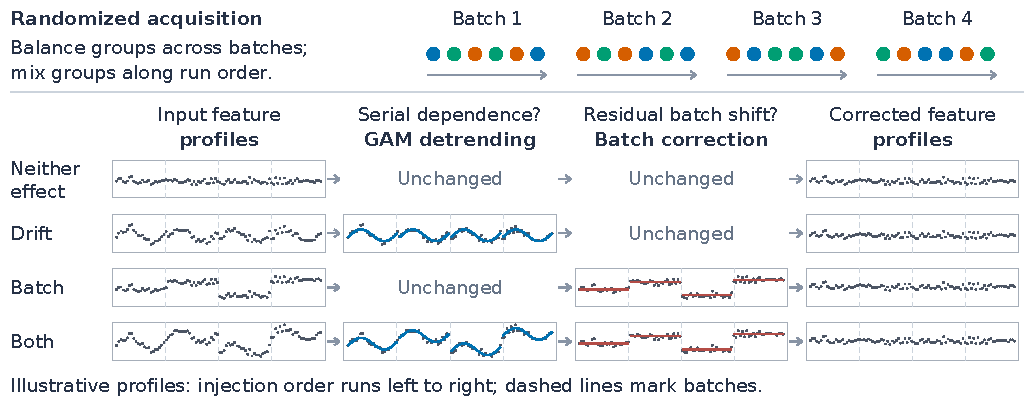
\includegraphics[width=\textwidth]{figures/F1_winn_overview.pdf}
\caption{\textbf{Overview of the WiNN workflow: randomize $\rightarrow$ test $\rightarrow$ correct.} Samples are balanced across batches and randomized along acquisition order. WiNN tests each feature within each supplied batch or inferred run segment, applies detrending only to those with detectable run-order drift, then applies residual batch correction only to features with a significant batch effect. MAD preparation and optional PQN are not shown.}
\par\smallskip{\footnotesize\textbf{Alt text:} Randomized acquisition is followed by tests for run-order and batch effects, with correction applied to selected features.\par}

\label{fig:winn-workflow}
\end{figure*}

\subsection{WiNN implementation and configurations}

All WiNN corrections used R package development version 0.1.7.9999. We benchmarked three configurations. \emph{WiNN}, our primary configuration, uses supplied batch labels without QC identities, adaptive-lag Ljung--Box statistics with permutation maxT adjustment at a familywise threshold of 0.05, ANOVA-based residual batch correction at a BH threshold of 0.05 and conservative PQN, with no parameter search. \emph{WiNN (QC-tuned)} also uses supplied batch labels and labeled training QCs to select parameters from a prespecified grid. \emph{WiNN (inferred segments)} combines QC-guided parameter selection with automatic inference of contiguous run segments and provides a fallback when batch labels are unavailable. All modes use the permutation gate and fit drift to all injections. Its guarantee does not extend to QC-guided selection or inferred segmentation. We recommend using recorded batch labels when available, because inferred batches do not consistently reproduce the recorded batch structure.

\subsection{Simulation studies}

We ran ten simulation seeds, each containing 1,000 features and 500 injections arranged in five plates of 100, including 450 study injections and 50 regularly interleaved pooled QCs, of which ten were held out as label-blinded evaluation references. Ground-truth log intensities were corrupted by feature-specific plate offsets and linear, nonlinear, autoregressive or mixed drift trajectories; the ground-truth matrix was used only for evaluation (Supplementary Methods S2).

To examine sensitivity to departures from randomization, we added a balanced binary phenotype to the study injections, with case-control log effects of $+0.35$ or $-0.35$ in 100 features and no effect in the remaining 900. Labels were withheld from correction and progressively aligned with batch, early within-plate run order or both. Maximum alignment means the strongest arrangement possible under this balanced design; it does not imply complete confounding. Effect recovery was the median corrected-to-ground-truth phenotype coefficient ratio across responsive features, with both coefficients adjusted for plate and within-plate position. Detection sensitivity and the false-discovery proportion were calculated after Benjamini--Hochberg adjustment at 5\%. This experiment tests one additive, two-group scenario rather than a general limit of identifiability.

\subsection{Empirical datasets}

We evaluated WiNN across four public datasets (Supplementary Table S1). MTBLS79 contains repeated cow and sheep heart measurements across eight analytical batches \citep{Kirwan2014DIMSBenchmark}. BatchCorr Set~1 contains repeated measurements of \emph{Arabidopsis} plant lines across ten batches \citep{Wehrens2016BatchCorr}. WaveICA contains human plasma metabolomics profiles with biological group labels \texttt{group\_0} and \texttt{group\_1}; their clinical meaning is unspecified in the benchmark metadata \citep{Deng2021WaveICA}. Sacurine contains urine metabolites and age, body mass index (BMI) and gender covariates \citep{Thevenot2015Sacurine,Thevenot2018W4M00001}.

We also evaluated WiNN on an internal clinical serum cohort acquired by flow-injection analysis MS (FIA-MS) \citep{Fuhrer2011FIATOF}. Study samples were randomized across 96-well plates under explicit balancing constraints, with pooled QCs and NIST1950 reference serum included throughout acquisition. Each biological sample was split into aliquots prepared on separate plates, and each preparation was measured in two consecutive technical injections. These adjacent measurements were averaged after $\log(1+x)$ transformation before correction. No phenotype or disease endpoint from this unpublished cohort was used (Supplementary Methods S2).

\subsection{Comparators, endpoints and uncertainty}

We compared raw data and WiNN with ComBat \citep{Johnson2007ComBat}, QC-RLSC \citep{Dunn2011}, QC-RFSC \citep{Luan2018StatTarget}, TIGER \citep{Han2022TIGER} and SERRF \citep{Fan2019SERRF}, with comparator settings selected using training QCs only (Supplementary Tables S2 and S3). Study-sample ANCOVA \citep{Wehrens2016BatchCorr} and mean-only batch centering provided baselines using the same intensity, order and batch information as WiNN.

Technical correction was assessed by held-out QC CV: the mean, across metabolites, of the standard deviation divided by the mean intensity in evaluation QCs, expressed as a percentage. QC labels were withheld from correction, although their profiles remained in the input matrix. Residual run-order drift measures the mean deviance explained by a smooth regression of $\log(1+x)$ intensity on run order within each metabolite-segment profile. Variance explained by batch summarizes batch association in the first five principal components (PCs), weighting each PC's $R^2$ by its variance. The same calculation measures variance explained by biological groups or covariates. These relative summaries describe the leading PCs, not total biological variance.

In simulation, ground-truth root mean squared error (RMSE) measures the discrepancy between corrected and ground-truth $\log(1+x)$ intensities. Feature-profile intraclass correlation, ICC(A,1), measures absolute agreement across samples and penalizes systematic shifts and rescaling that Pearson correlation can miss \citep{McGrawWong1996}; sample-profile Pearson correlation measures agreement with ground truth across metabolites within each sample. For empirical replicates, ICC(A,1) measures agreement between separately acquired profiles of the same biological sample. Cross-batch sample matching asks whether a profile's most correlated match in another batch comes from the same sample. Biological group effects were also assessed feature by feature. Uncertainty used 2,000 paired bootstrap draws of biological samples (plant lines in BatchCorr), carrying repeated measurements together and using the same draws for every method. These intervals condition on the fitted correction; clinical resampling is by sample, not patient. Association counts were compared with 5,000 design-constrained permutations \citep{EfronTibshirani1993,FreedmanLane1983}. Supplementary Methods S4 gives dataset-specific resampling rules and full endpoint definitions.

\section{Results}
\label{sec:results}

\subsection{WiNN recovers ground-truth profiles in randomized simulations}

We first used simulated data with known ground truth to verify that WiNN removed simulated technical variation while preserving the underlying metabolite and sample profiles. Across ten paired simulations, WiNN reduced mean held-out QC CV from 44.55\% to 8.88\% and residual run-order drift from 12.51\% to 3.31\%. Ground-truth RMSE fell from 0.293 to 0.074, feature-profile ICC(A,1) increased from 0.588 to 0.919 and sample-profile correlation increased from 0.519 to 0.920 (Figure~\ref{fig:simulation}B--D). WiNN ranked ahead of every primary comparator on each of the three truth endpoints in all ten seeds, and it also improved all three endpoints over mean-only batch adjustment and study-sample ANCOVA (RMSE 0.116 and 0.098) in every seed (Supplementary Tables S4 and S11).

The partial-confounding study showed how biological recovery changed as randomization was weakened. With randomized phenotype labels, WiNN recovered a median 0.961 of the ground-truth case-control effect and detected all 100 responsive features. Batch alignment had little effect on coefficient recovery because one plate remained balanced even at maximum alignment, permitting plate-adjusted estimation, although detection sensitivity fell to 0.882 at maximum batch alignment. Strong run-order alignment attenuated recovery to 0.866 of the ground-truth effect, and joint alignment was most severe: at maximal joint alignment, ground-truth effect recovery fell to 0.740, detection sensitivity to 0.507 and the mean false-discovery proportion rose to 0.359 (Figure~\ref{fig:simulation}E,F). Across the alignment grid, WiNN's held-out QC CV remained between 9.00\% and 9.84\% and its residual run-order drift between 3.3\% and 4.2\% (Supplementary Table S7), showing that low residual technical variation can coexist with attenuated biological effects and inflated false discoveries when randomization fails.

\begin{figure*}[t]
\centering
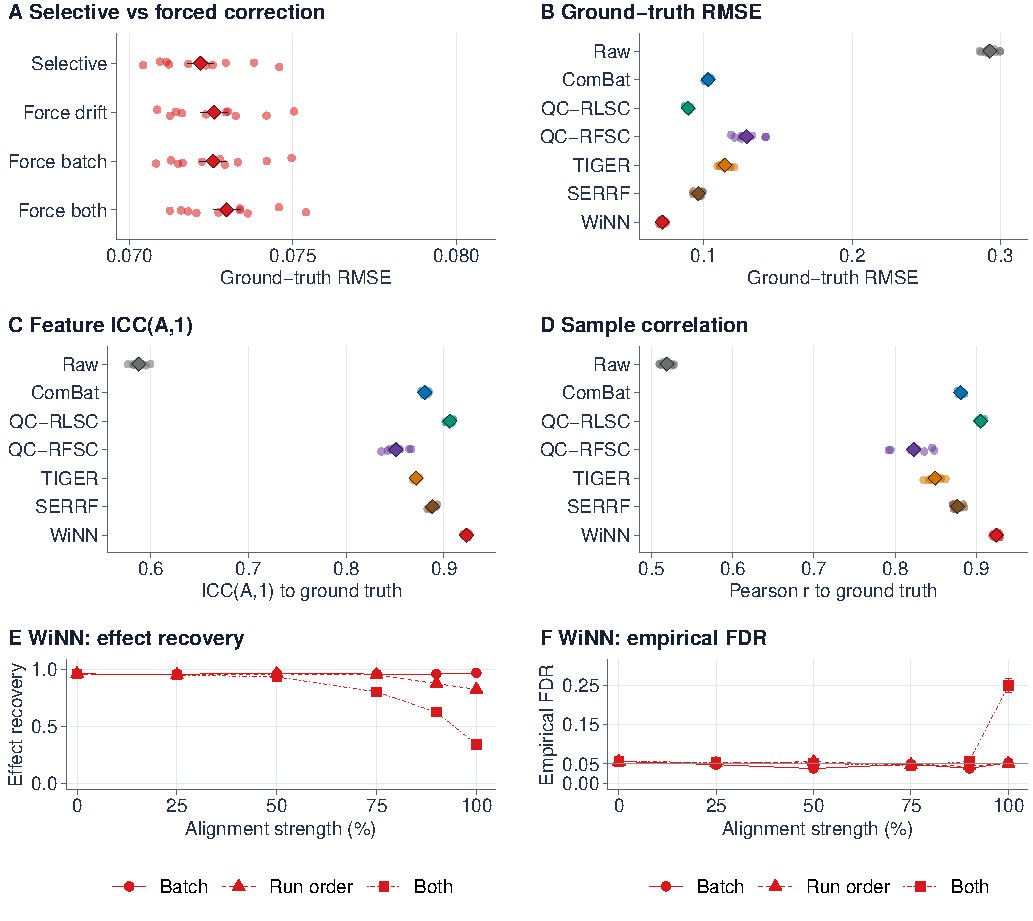
\includegraphics[width=\textwidth]{figures/F2_simulation.pdf}
\caption{\textbf{Ground-truth recovery and sensitivity to confounding.} (A) Ground-truth RMSE for selective versus forced correction. (B--D) Seven primary methods across ten seeds; diamonds and bars are means and standard errors. Lower values are favorable in A and B and higher values in C and D. (E) Median corrected-to-ground-truth phenotype-effect ratio among 100 responsive features and (F) mean false-discovery proportion (grey line, nominal 0.05) as phenotype is aligned with batch, run order or both; 100\% is the maximum feasible alignment in this design, not complete confounding. Points and bars are means and standard errors across ten seeds.}
\par\smallskip{\footnotesize\textbf{Alt text:} Among the seven primary methods, WiNN has the lowest simulation error and highest truth agreement. Strong phenotype alignment with acquisition order can reduce biological recovery despite low technical variation.\par}
\label{fig:simulation}
\end{figure*}

\subsection{WiNN improves agreement between repeated sample measurements}

BatchCorr tested whether correction preserves differences between samples, using repeated measurements of the same \emph{Arabidopsis} plant lines across batches. WiNN reduced held-out QC CV from 66.57\% to 27.30\%, residual run-order drift from 12.24\% to 5.54\% and variance explained by batch from 56.11\% to 0.062\%, while replicate ICC(A,1) increased from 0.885 to 0.952 (Figure~\ref{fig:replicates}A,C). Cross-batch sample matching increased from 46.3\% to 71.4\%, similar to ComBat (71.6\%) and QC-RLSC (71.3\%) (Supplementary Table S10).

The internal clinical FIA-MS cohort provided complementary evidence, as each biological sample was measured repeatedly across plates and NIST1950 reference serum was available for separate assessment of technical precision. WiNN reduced held-out QC CV (NIST1950) from 16.59\% to 12.03\%, residual run-order drift from 12.03\% to 9.34\% and variance explained by plate from 15.05\% to 0.221\%, while replicate ICC(A,1) increased from 0.9810 to 0.9898 (Figure~\ref{fig:replicates}B,D). WiNN had the lowest held-out QC CV (NIST1950) among the seven primary methods; TIGER had the lowest residual run-order drift (9.03\%). Cross-plate sample matching increased from 75.2\% to 85.8\%, with TIGER reaching the highest accuracy (88.1\%).

\begin{figure*}[t]
\centering
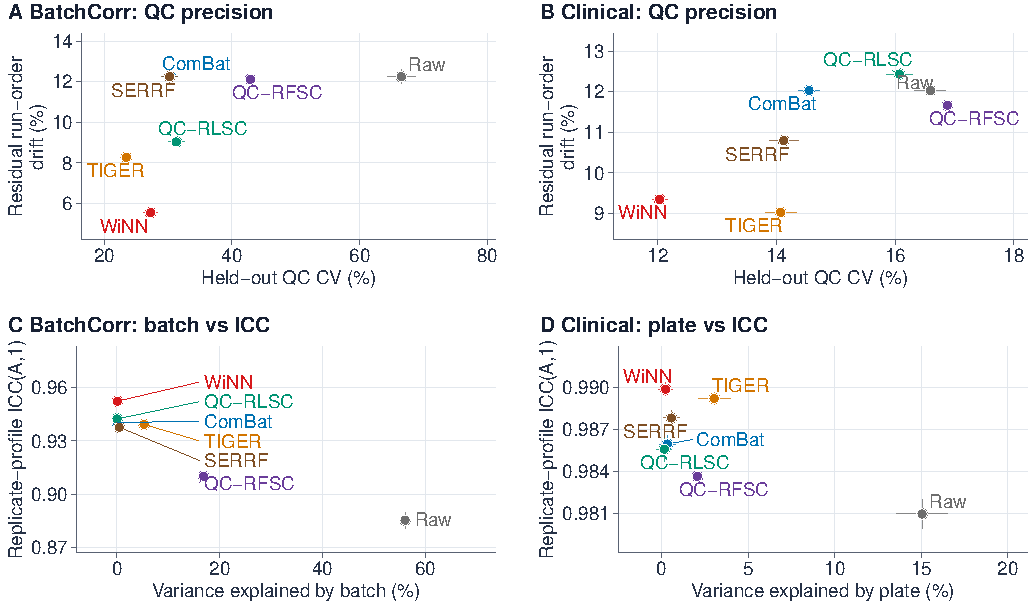
\includegraphics[width=\textwidth]{figures/F3_replicates.pdf}
\caption{\textbf{Technical correction and replicate agreement.} (A,B) Held-out QC CV versus residual run-order drift (percentages) in BatchCorr and the clinical cohort; bars are standard errors across features or feature-segment profiles. (C,D) Variance explained by batch or plate versus replicate ICC(A,1); bars are bootstrap standard errors from 2,000 resamples of biological samples. QC-RFSC points have no recomputed uncertainty. Lower x and higher y are favorable in C and D.}
\par\smallskip{\footnotesize\textbf{Alt text:} WiNN reduces held-out QC variability and batch structure and increases replicate agreement in the plant and clinical datasets; comparator rankings vary by endpoint.\par}
\label{fig:replicates}
\end{figure*}

\subsection{WiNN retains biological group structure}

WaveICA had strong batch separation and weaker biological group differences. WiNN reduced variance explained by batch from 69.44\% to 0.284\%, while variance explained by biological group increased from 0.277\% to 1.352\% (Figure~\ref{fig:public-biology}A). ComBat, QC-RLSC and SERRF removed most batch separation but retained less relative group association than WiNN, whereas TIGER and QC-RFSC retained about three quarters of the raw batch association. The group labels support this statistical comparison, but do not establish a specific clinical interpretation.

MTBLS79 provided a known cow-sheep contrast across repeated analytical batches. WiNN reduced variance explained by batch from 36.10\% to 1.088\%, while variance explained by species changed from 43.54\% to 44.21\% (Figure~\ref{fig:public-biology}B). Among 2,488 tested features, 1,097 differed between species after WiNN correction at BH-adjusted $P<0.05$, compared with 1,075 before correction (Supplementary Table S8). Both counts exceeded the design-constrained permutation null. These counts indicate a strong biological contrast; without feature-level ground truth, more discoveries do not by themselves establish better correction. ComBat and SERRF also retained strong species separation. Sacurine age, BMI and gender results varied by covariate (Supplementary Tables S4 and S8).

\begin{figure*}[t]
\centering
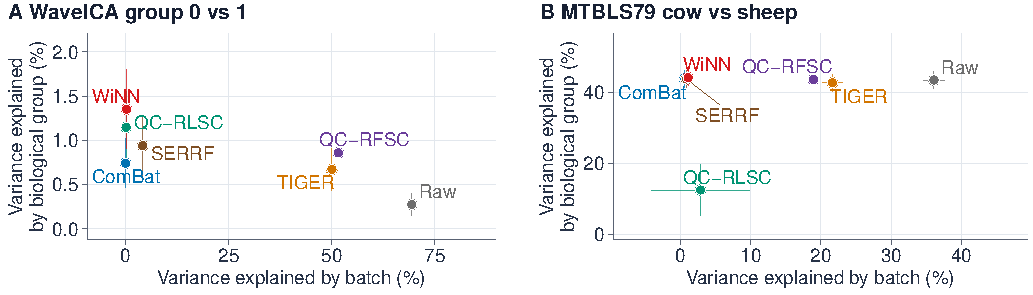
\includegraphics[width=\textwidth]{figures/F4_biological_structure.pdf}
\caption{\textbf{Biological group structure after correction.} (A) WaveICA variance explained by batch versus biological group. (B) MTBLS79 variance explained by batch (134 injections) versus species (20 extracts after averaging repeated measurements). Both axes summarize the first five PCs. Bars are bootstrap standard errors from 2,000 stratified resamples; QC-RFSC points have no recomputed uncertainty. Lower x and higher y are favorable.}
\par\smallskip{\footnotesize\textbf{Alt text:} WiNN reduces batch association in WaveICA and MTBLS79 while retaining relative biological group association.\par}
\label{fig:public-biology}
\end{figure*}

\subsection{Effects of selective correction}

We examined each correction step and compared selective correction with correcting every eligible profile. Batch adjustment accounted for the largest reductions in held-out QC CV and variance explained by batch in most datasets; detrending primarily reduced residual run-order drift (Supplementary Figure S1). Correcting drift in every testable profile reduced this drift measure further but increased held-out QC CV in four of six datasets, improving it only in BatchCorr and Sacurine (Supplementary Table S6). Forcing drift correction while keeping batch correction selective gave lower ground-truth RMSE (0.0726 versus 0.0744) and higher feature ICC and sample correlation in all ten simulations (Figure~\ref{fig:simulation}A). Forcing batch adjustment had mixed effects; WiNN already selected 72.5--98.0\% of eligible features for this step.

\subsection{Limits of the selection test and preprocessing}
\label{sec:stress}

We tested whether WiNN selects features when no technical drift is present. In 1,000 experiments with 100 independent null features at each segment length, MAD preparation followed by permutation maxT selection at 5\% selected at least one feature in 4.0\%, 3.9\%, 4.8\% and 4.5\% of experiments with 20, 50, 100 and 200 injections, respectively (Supplementary Figure S11). Under this global null, familywise error and FDR coincide. The legacy asymptotic Ljung--Box/BH gate gave 13.5\%, 34.9\%, 19.8\% and 12.3\% on the same data. Calibration depends on exchangeable order: periodically interleaved reference and study samples with different mean intensities still triggered selection without drift. Separately, MAD preparation and PQN together retained ground-truth effect ratios of 1.000 for balanced sparse responses, 0.310 for a rare-subgroup response and 0.534 for a widespread coordinated response (Supplementary Table S12). Selective drift and batch correction cannot prevent signal loss introduced by these preprocessing steps.

\section{Discussion}
\label{sec:discussion}

WiNN combines tests for run-order and batch effects with conservative correction of selected features. It recovered ground-truth profiles in simulation and improved technical precision and replicate agreement across the empirical benchmarks. No method was best on every endpoint. Forced detrending gave slightly better ground-truth recovery in these simulations, illustrating the sensitivity cost of conservative selection.

The results reinforce the need to evaluate biological preservation alongside technical precision. Low held-out QC CV and little residual run-order drift can coexist with attenuated biological effects and increased false discoveries. In our confounding experiment, this occurred when phenotype was aligned with both batch and run order. The apparent tolerance to batch alignment depended on remaining within-batch overlap and should not be interpreted as protection against complete confounding. The simulations cover additive effects of one size in a balanced two-group design; other effect sizes, abundance distributions and dependence structures may behave differently.

WiNN does not require QC labels in its primary configuration, but QCs remain useful for monitoring acquisition and independently evaluating correction. Recorded batch labels should be used when available, since automatic segmentation did not consistently recover documented boundaries. Reference placement also matters: periodically interleaved sample types can create serial dependence unrelated to instrumental drift. Permutation calibration reduced excess false selection in these null experiments, but its guarantee requires exchangeable profiles within prespecified segments and does not extend automatically to QC-guided tuning or inferred segmentation. In addition, MAD shrinkage can attenuate rare biological responses, and PQN can remove widespread coordinated shifts. These limitations should guide the choice of preprocessing and the interpretation of corrected data.

Runtimes are reported by dataset and configuration in Supplementary Table S5. The fixed configuration avoids parameter search. Together with support for data acquired by different MS workflows, this makes it useful for studies with reliable acquisition metadata but limited QC annotation. Accounting for nonexchangeable sample structures and for selection of segments or tuning parameters remains a priority for further development. The present evidence supports selective correction as a practical approach under suitable experimental designs, with biological validation needed for each new application.

\section*{Supplementary data}
Supplementary data are available at \textit{Bioinformatics} online.

\section*{Data availability}
The WiNN analyses used development version 0.1.7.9999 (GPL-3; commit \texttt{ab49697}) at \url{https://github.com/ratschlab/winn}. CRAN version 0.1.6 (\url{https://CRAN.R-project.org/package=winn}; DOI: \nolinkurl{10.32614/CRAN.package.winn}) predates this calibration. Simulation, data-retrieval and analysis code and numerical inputs are fixed at \href{https://github.com/ratschlab/WiNN-for-technical-correction/tree/3794b8408070950cd59c0eed9fe207c6c8fbb5f6}{analysis revision 3794b840}; final figures, tables and generators are in the \href{https://github.com/ratschlab/WiNN-for-technical-correction/tree/main/manuscript}{manuscript bundle}. The internal clinical metabolomics data will be released with a forthcoming manuscript describing the cohort; aggregate results supporting the present analyses accompany the reproducibility package.

\section*{Funding}
This work was supported in part by institutional funding and grants from the Swiss Cancer League (Krebsliga; KLS-5463-08-2021 to G.R.) and the Swiss National Science Foundation (SNSF; grant 213236 to A.K.).

\section*{Acknowledgements}
We thank the Zamboni group at ETH Zürich for performing the FIA-MS measurements for the clinical cohort and for preprocessing the data to generate the raw metabolite intensity matrix. OpenAI Codex was used to assist manuscript editing, code implementation and validation.

\section*{Author contributions}
T.T. led conceptualization, formal analysis, methodology, software and original drafting, and supported funding acquisition. Y.Z. supported formal analysis, methodology and software; A.S. and A.J. supported methodology and software; F.G. supported conceptualization; M.L. supported conceptualization and methodology. A.K. contributed equally to funding acquisition, M.P.L. supported it, and G.R. led it and contributed equally to supervision. O.D. contributed equally to conceptualization and methodology and led supervision.

\section*{Conflict of interest}
The authors declare no conflicts of interest.

\begingroup
\footnotesize
\setlength{\bibsep}{0pt}
\bibliographystyle{oup-abbrvnat}
\bibliography{references}
\endgroup

\end{document}
